\documentclass[a4paper,10pt]{article}
\usepackage{titling}
\usepackage{fullpage}
\usepackage{times}
\usepackage{graphicx}
\usepackage{multicol}
\usepackage{float} %to place tables properly
\usepackage{placeins} %to place tables properly
\usepackage{fancyhdr} % Package to make headers 
\usepackage{soul}% Package for highlights
\usepackage{enumitem}% Package to make lists
\usepackage{geometry}% Package for margin adjusting
\usepackage[table]{xcolor}% Package for table colors
\usepackage[hidelinks]{hyperref}
\usepackage{multirow}
\usepackage{listings} % Package to insert code
\usepackage{titlesec} % Package to change title format


%°°°°°°°°°°°°°°°°°° LAYOUT AND COMMAND DEFINITION °°°°°°°°°°°°°°°°°°°°

\definecolor{pyblue}{RGB}{31,119,240}

\renewcommand{\headrulewidth}{0pt}

\geometry{
  left=2cm, % adjust the left margin
  right=2cm, % adjust the right margin
  top=2cm, % adjust the top margin
  bottom=2cm, % adjust the bottom margin
}

\titlespacing*{\subsection}{0pt}{12pt}{7pt}
\titlespacing*{\subsubsection}{0pt}{10pt}{2pt}


\graphicspath{{Figures/}}


%°°°°°°°°°°°°°°°°°°°°°DEFINE TITLE PAGE°°°°°°°°°°°°°°°°°°°°°°°°°°°°°°


\pretitle{
  \begin{center}
  \LARGE
  
\includegraphics[width=15.1cm,height=3.05cm]{Logo_unipv.png}\vspace*{1cm}\\[\bigskipamount]}


%Title structure
\title{\Large {Enterprise Digital Infrastructure Course} \vspace{0.2cm}
     \rule{\textwidth}{0.3pt} \vspace{0.0cm} % insert an horizontal line. Thickness 0.3pt
     \textbf{Web Services Performance} \vspace{0.0cm} %bold title
     \rule{\textwidth}{0.3pt}}

%information about author
\author{Andrea Alberti \vspace{0.1cm}\\
        \small Department of Computer Engineering - Data Science \vspace{0.2cm}\\
        \small University of Pavia, Italy \vspace{0.2cm}\\
        \small Contact: andrea.alberti01@universitadipavia.it\\
        \small GitHub: \small \url{https://github.com/AndreaAlberti07}}

\tiny \date{\today}

%°°°°°°°°°°°°°°°°°°°°°°DOCUMENT TITLE PAGE°°°°°°°°°°°°°°°°°°°°°°°°°°°°°°°°°

\begin{document}

%Insert a short summary of your lab activities.

\begin{titlepage}
        \maketitle 
        \thispagestyle{empty} 
\begin{multicols*}{2}

\hrule
\tableofcontents
\newcolumn
\hrule
\begin{abstract}
        \noindent
        This report presents an analysis of web services, focusing on their implementation aspects and the impact on their performance. 
The study examines several factors that influence performance, including the number of parallel TCP connections, caching mechanisms, 
HTTP versions, and warm-up time allocation.
The primary metric used to investigate the impact of these factors on the performance is the page load time (PLT). Additionally, the study aims to compare the performance of different websites under various conditions, 
utilizing metrics such as Requests Per Second (RPS), Time Per Request (TPR) and its Standard Deviation (SD).
Several tools were employed for data collection and analysis, including the Apache Benchmark, the Web Development Tools integrated into Mozilla Firefox, 
and the h2load tool. The experiments were performed multiple times within the same day to ensure accurate and consistent results.
The study highlights the optimal number of parallel TCP connections, showing the importance of caching mechanisms and  
the superiority of newer HTTP versions. Furthermore, the study identifies the potential impact of warm-up time allocation on web service performance.
Overall, this research contributes to the understanding and improvement of web service implementation and performance. 

\end{abstract}


        
\end{multicols*}
\end{titlepage}


\newpage
\listoffigures
\listoftables

\thispagestyle{empty}
\newpage
\begin{multicols}{2}
\clearpage
\setcounter{page}{1}

%°°°°°°°°°°°°°°°°°°°°°°°°°°°°°°°°°BEGIN BODY OF THE DOCUMENT°°°°°°°°°°°°°°°°°°°°°°°°°°°°°°°°


%°°°°°° General introduction and setup °°°°°°
\section{Introduction}
Internet technologies play a crucial role in modern society, facilitating seamless communication, information exchange, and collaboration 
over the internet. The continuous advancement of these technologies is shaping the way we live, work, and interact, transforming various
industries and providing new opportunities for growth and connectivity. One of the most important branches of Internet Technologies 
are the Web Services. This report is aimed at the analysis of the performance of these services,
focusing on their implementation aspects and the impact on their performance.
\section{Experimental Setup}
\label{sec:experimental_setup}
\begin{itemize}[leftmargin=9pt]
\item \textbf{Why}: The first goal involves investigating the impact of the number of parallel connections, caching policies and HTTP version on the PLT. The second goal is to compare different websites 
in different conditions to asses their performance.
\item \textbf{Which}: The used websites are listed in table \ref{tab:websites}.
\item \textbf{What}: The metrics used are the PLT for the first goal, while RPS and TPR are used for the second one.
\item \textbf{Where}: The experiments are conducted with a Macbook Pro 14, equipped with a Virtualized Ubuntu 22.04 LTS.
The browser is \textit{Mozilla Firefox} and the internet connection is a FTTH 200/20 Mbps provided by Vodafone IT.
\item \textbf{How}: The used tools are the \textit{Apache Benchmark}, the \textit{Web Dev. Tools} built-in in Mozilla Firefox and \textit{h2load tool}.
\item \textbf{When}: The experiments are conducted several times in the same day to provide reliable results.
\end{itemize}

\begin{table}[H]
    \small
    \centering
    \rowcolors{2}{pyblue!25}{white}
    \begin{tabular}{|c|c|}
    \hline
    \rowcolor{pyblue!60}
    \textbf{Website} & \textbf{URL} \\ \hline
    Apple & \url{https://www.apple.com/store} \\ 
    Harvard & \url{https://www.harvard.edu/} \\ 
    MIT & \url{https://www.mit.edu/} \\ 
    V.News & \url{https://www.vallesabbianews.it/} \\ 
    GZ & \url{https://www.grafichezorzi.it/} \\ 
    V.Spluga & \url{https://vallespluga.it/} \\ 
    Unitus & \url{http://www.unitus.it/} \\ 
    MIT gov & \url{https://www.mit.gov.it/} \\ 
    Istat & \url{https://www.istat.it/} \\ 
    OffWhite & \url{https://www.off---white.com/}\\ \hline
    \end{tabular}
    \caption{\small List of tested websites}
    \label{tab:websites}
\end{table}




%°°°°°° Web Services °°°°°°
\section{Web Services}
The increasing frequency of user interactions with websites has brought to light the criticality of website performance 
in delivering a satisfactory user experience. Among the key performance factors, page load time holds significant importance. 
To optimize this aspect, an option is to focus on managing the number of parallel connections exploitable between client and server,
and implementing effective caching policies. The ultimate objective is to minimize page load time (PLT), thus 
fostering user engagement and ensuring an enhanced user experience.
\subsection{Parallel TCP}
The number of parallel connections refers to a browser's ability to establish simultaneous connections to retrieve 
multiple resources concurrently. Increasing parallel connections can potentially expedite page load times, but it may 
also strain server resources and lead to network congestion. Specifically:

\begin{itemize}[leftmargin=10pt]
\item \textbf{Fewer Parallel Connections}: If the number of parallel connections is set too low, it can result in
 slower page load times. With fewer connections, the browser fetches resources sequentially, causing delays as it waits
 for each request to complete before initiating the next one.
\item \textbf{Default Number of Parallel Connections}: Most modern browsers allow around six parallel connections per
 host by default. This number hit a balance between resource fetching and the server's load. With this setting, the 
 browser can fetch multiple resources simultaneously, improving the overall page load performance. 
\item \textbf{Higher Number of Parallel Connections}: Increasing the number of parallel connections can potentially
 speed up page load times. By allowing more simultaneous connections, the browser can fetch a greater number of 
 resources in parallel, reducing the overall loading time. However, an excessively high value may overwhelm the 
 server and cause network congestion.
\end{itemize}
\noindent
This section presents a practical investigation into the influence of the number of parallel connections on the Page Load Time (PLT). 
Various websites (as listed in Table \ref{tab:websites_details}) were tested using different numbers of parallel connections 
to determine the configurations that benefit the most from parallel TCP connections.

    \begin{table}[H]
        \small
    \centering
    \rowcolors{2}{pyblue!25}{white}
        \begin{tabular}{|l|c|c|}
        \hline
        \rowcolor{pyblue!60}
        \textbf{Website} & \textbf{Number of Objects} & \textbf{Size (MB)} \\
        \hline
        Vallesabbia & 118 & 5.01 \\
        Grafiche & 65 & 5.31 \\
        Vallespluga & 151 & 20.03 \\
        Unitus & 72 & 1.74 \\
        Gov & 218 & 9.98 \\
        Istat & 134 & 11.33 \\
        \hline
        \end{tabular}
        \caption{\small Websites details}
        \label{tab:websites_details}
    \end{table}


Before each measurement, the browser cache was cleared and the "disable cache" option in Mozilla Web Developer Tools was enabled. 
The selection of tested sites was conducted carefully to utilize the HTTP/1.1 protocol, which allows for the utilization of multiple parallel TCP connections. 
This choice aimed to highlight the potential benefits that can be derived from employing such connections. Each website was tested using different numbers of 
TCP connections, specifically 1, 5, 10, and 15. To ensure accurate measurements, the reported Page Load Time (PLT) represents the average value obtained 
from five data points collected under the same experimental conditions.
It is important to note that the actual number of TCP connections established depends on the server configuration, as the client merely expresses its preference. 
To ensure proper interpretation of the results, the number of opened TCP connections was verified using Wireshark, and these details are provided 
in Table \ref{tab:TCP_asked}.

    \begin{table}[H]
        \small
    \centering
    \rowcolors{2}{pyblue!25}{white}
        \begin{tabular}{|l|c|c|}
        \hline
        \rowcolor{pyblue!60}
        \textbf{Website} & \textbf{N. TCPs Ask} & \textbf{N. TCPs Estab.} \\
        \hline
        Vallesabbia & 15 & 15 \\
        Grafiche & 15 & 13 \\
        Vallespluga & 15 & 15 \\
        Unitus & 15 & 15 \\
        Gov & 15 & 15 \\
        Istat & 15 & 15 \\
        \hline
        \end{tabular}
        \caption{\small Number of TCP connections asked and established}
        \label{tab:TCP_asked}
    \end{table}

Analysis of Figure \ref{fig:plt_n_tcp} reveals a decrease in PLT as the number of connections increases. However, this trend only persists until a certain threshold 
(in this case, 5 connections), beyond which the PLT remains relatively constant. The specific reasons for this behavior are not apparent from the conducted 
experiments, as the servers configuration remains unknown, resembling a black box. Notably, the website that derives the most benefit from concurrent TCP 
connections is \textit{Istat}. This advantage is not solely attributable to the size of the website or the number of objects it contains, as other 
websites with larger sizes exhibit a different behavior. Therefore, further investigations are necessary to identify the underlying factors contributing 
to this phenomenon.
Overall, it can be concluded that the number of parallel TCP connections significantly impacts the PLT. However, the benefits tend to plateau as the number of 
connections increases excessively. The default choice of six concurrent TCP connections made by the browser appears to be a reasonable selection based on the 
findings of this study.
    
    \begin{figure}[H]
        \centering
        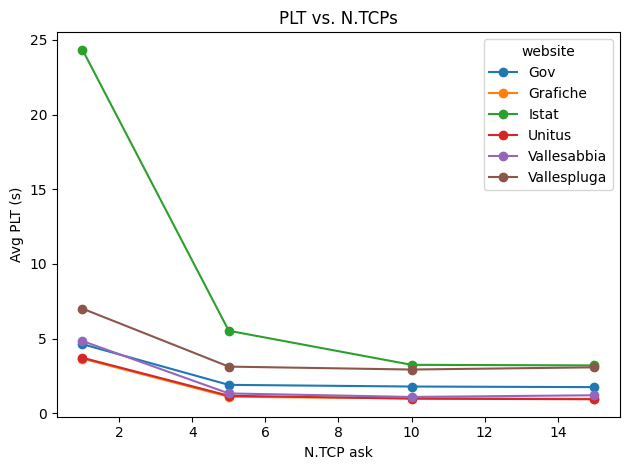
\includegraphics[width=0.48\textwidth]{1_plt_n_tcp.png}
        \caption{\small Page Load Time (PLT) vs. N.TCP}
        \label{fig:plt_n_tcp}
    \end{figure}




\subsection{Caching Policy}
Caching policies, controlled through HTTP headers, significantly impact page load times by reducing the need for repeated 
resource requests. Effective caching policies leverage client-side (browser caching) and intermediate server storage 
(proxy caching). \\
\\
\textbf{Proxy caching} involves storing copies of web resources at intermediate proxy servers, which can then serve subsequent requests 
for the same resources without contacting the origin server. This reduces network latency and bandwidth usage.\\
\\
\textbf{Browser caching} involves storing web resources locally on the client's device, allowing subsequent page visits to be loaded 
faster without the need to re-download the same resources.\\
\\
\textbf{Implementation}: the implementation of caching policies is facilitated through the use of the 'Cache-Control' header in HTTP responses. 
This header allows servers to communicate specific caching directives to clients and intermediaries. It provides instructions such as the maximum 
time a resource should be considered fresh ('max-age') and whether the resource can be cached by intermediate proxies ('public') or the browser ('private').
To ensure the validity of cached resources, several headers are utilized in caching strategies. The 'Expires' header specifies the date and time after which 
the resource should be considered stale. The 'Last-Modified' header indicates the date and time of the resource's last modification. Additionally, 
the 'ETag' header provides a unique identifier for the resource. These headers enable three main non-mutually exclusive strategies for validating 
cached resources: 'Expiration', 'Validation', and 'Heuristic'. The \textbf{Expiration} and \textbf{Heuristic} strategies generally result in faster response times, 
as they rely on pre-determined expiration dates or heuristics to determine the freshness of the cached resources. On the other hand, 
the \textbf{Validation} strategy requires a round-trip to the server to confirm the validity of the cached resources, resulting in slower response times.

\subsubsection{Caching mechanisms}
To evaluate the impact of caching policies on page load times, various websites with different caching strategies leveraging the browser cache were tested. 
The results, as depicted in Figure \ref{fig:2_site_policy}, clearly demonstrate the benefits of caching. Enabling caching led to a significant reduction 
in page load times across all tested websites. 

    \begin{figure}[H]
        \centering
        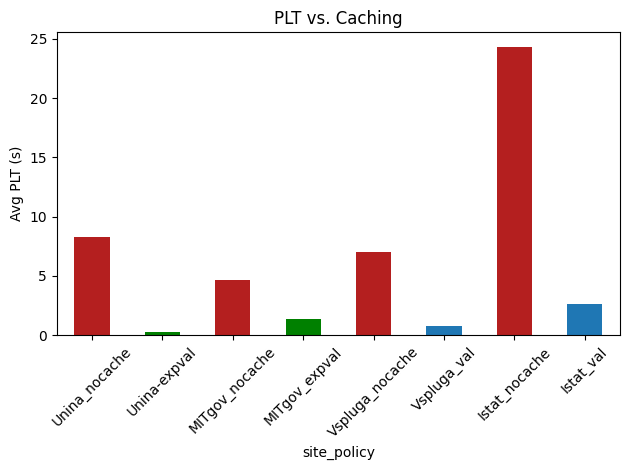
\includegraphics[width=0.48\textwidth]{2_site_policy.png}
        \caption{\small Caching policies of the tested websites}
        \label{fig:2_site_policy}
    \end{figure}

Interestingly, when comparing the specific methods used to validate cached resources (validation and exp+validation), no noticeable differences were observed (Figure \ref{fig:2_policy}).
This observation can be attributed to two factors. Firstly, websites can implement different caching policies for various resources, making it challenging 
to discern distinct impacts on page load times. Secondly, the performance gap between the 'Expiration' and 'Validation' strategies primarily arises 
when the resources are cached and not yet expired, allowing the 'Expiration' strategy to be leveraged. However, verifying this fact requires a thorough 
examination of individual resources, which is not easily feasible.

    \begin{figure}[H]
        \centering
        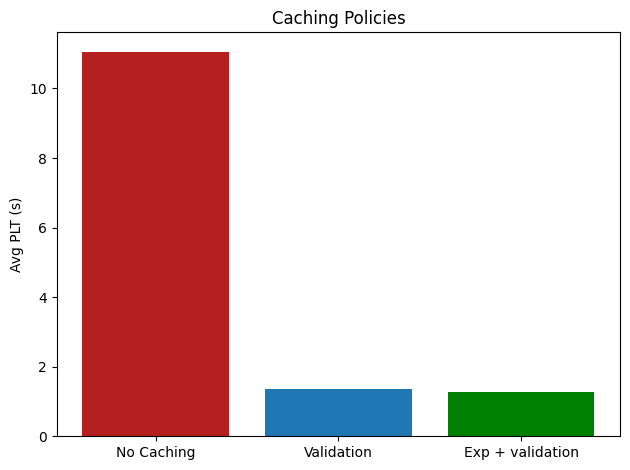
\includegraphics[width=0.48\textwidth]{2_policy.png}
        \caption{\small Page Load Time (PLT) vs. Caching Policy}
        \label{fig:2_policy}
    \end{figure}

In conclusion, even though the 'Expiration', 'Validation', and 'Heuristic' strategies have their advantages and trade-offs, the overall performance 
benefits of caching are evident.

\subsubsection{Caching and HTTP version}
Over the years, multiple versions of the HTTP protocol have been released, each introducing new features and improvements. 
HTTP/1.1 brought advancements such as persistent connections, pipelining, and caching. These enhancements aimed to enhance the efficiency 
of resource delivery. Building on this foundation, HTTP/2 introduced significant improvements, including binary framing, multiplexing, server push, 
and header compression. These features further optimized the protocol's performance.
HTTP/3, the latest version, introduced a new transport protocol called QUIC, which is based on UDP (User Datagram Protocol), as opposed to 
the previous versions that relied on TCP (Transmission Control Protocol). This change in the underlying transport protocol offers potential benefits such as 
improved latency, better congestion control, and enhanced security.
Despite these protocol advancements, the fundamental caching system remains unchanged and relies on headers.
To practically assess the performance impact of different HTTP versions and the influence of caching, a website (Off-White) was subjected to 
testing. The website was tested using different versions of the HTTP protocol, with caching enabled and disabled. The experimental results are depicted 
in Figure \ref{fig:3_version_caching}.

    \begin{figure}[H]
        \centering
        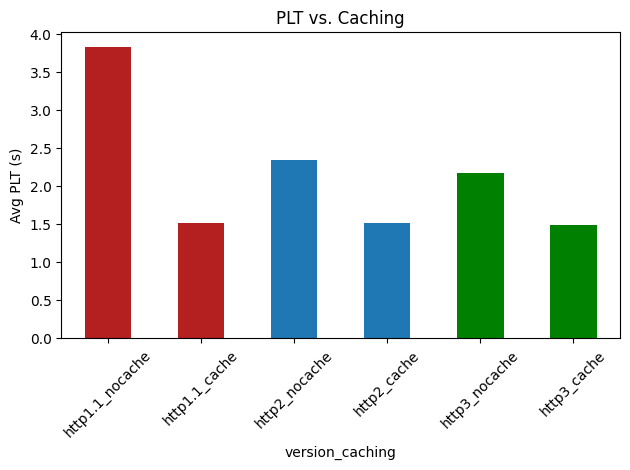
\includegraphics[width=0.48\textwidth]{3_version_caching.png}
        \caption{\small Page Load Time (PLT) vs. HTTP version and caching}
        \label{fig:3_version_caching}
    \end{figure}

As anticipated, enabling caching resulted in a substantial decrease in page load times for all tested versions of the HTTP protocol. 
The uniformity of loading times with caching enabled suggests that the caching mechanism played a more prominent role in influencing performance than the 
specific protocol version being used. This underscores the significance of efficient caching strategies in optimizing overall page load times.\\
Another interesting observation is depicted in Figure \ref{fig:3_version}. As expected, each new protocol version outperforms the previous one.
This performance improvement is not dependent on caching mechanism and it is attributable to the above discussed enhancements brought by each new version.

    \begin{figure}[H]
        \centering
        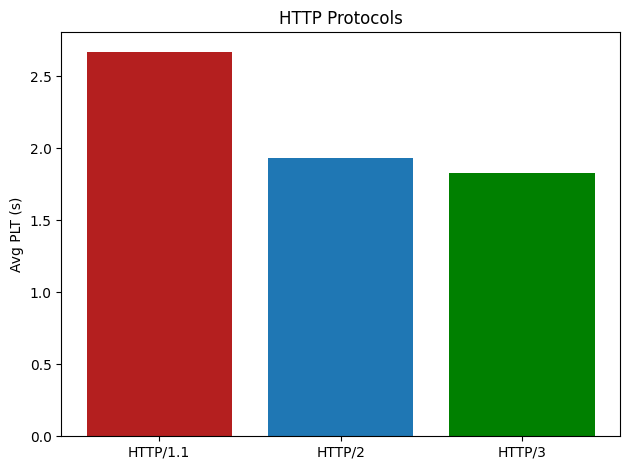
\includegraphics[width=0.48\textwidth]{3_version.png}
        \caption{\small Page Load Time (PLT) vs. HTTP version}
        \label{fig:3_version}
    \end{figure}

\subsection{Performance}
This section presents a comparative analysis of the performance of three distinct websites. To gain insights into their performance under different 
conditions, two key parameters (Figure \ref{fig:4_tuples}) were varied throughout the experiments: the number of requests sent to each website and the concurrency level. 
It is important to note that these parameters' values were chosen conscientiously, taking ethical considerations into account to prevent overloading the websites.
All experiments were conducted using identical conditions, as described in Section \ref{sec:experimental_setup}. The used scripts
can be consulted in Appendix \ref{sec:scripts}.

    \begin{figure}[H]
        \centering
        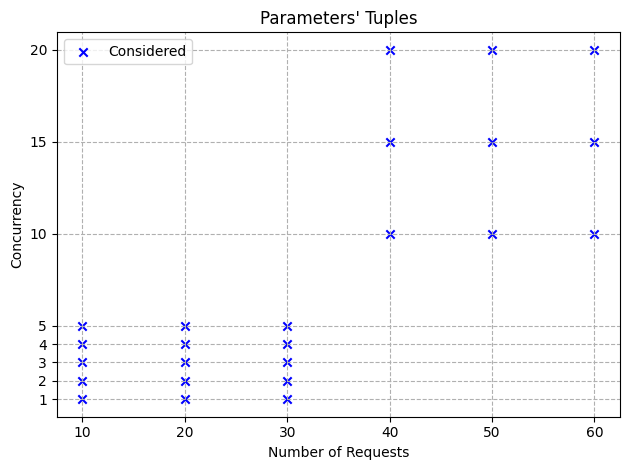
\includegraphics[width=0.48\textwidth]{4_tuples.png}
        \caption{\small Concurrency and RPS combinations}
        \label{fig:4_tuples}
    \end{figure}



It is worth mentioning 
that the client-side cache was intentionally disabled to ensure that the experiments accurately captured the website's performance without any caching effect.
All the results were gathered using the \textit{Apache Benchmark} tool, and the metric used to compare the websites is the RPS (Requests Per Second).
Three analysis are presented: the first one consider the impact on the RPS of the concurrency level, the second one the impact of the number of requests,
and the last the overall RPS achieved by each website.

\subsubsection{Concurrency VS RPS}
The concurrency is intended as the number of concurrent clients hitting the website at the same time. As the concurrency level increases, 
the website's server is required to process multiple requests concurrently. This can result in a higher 
RPS, as more requests are being handled simultaneously. However, there may be limits to the server's capacity 
to handle concurrent requests efficiently.
If the server is properly configured and equipped to handle the increased concurrency, it may exhibit a linear or near-linear increase in 
RPS as the concurrency level rises. 
However, there may be a point of diminishing returns where further increasing the concurrency level does not lead to a significant increase 
in RPS or may even negatively impact the server's performance. This can occur if the server becomes overwhelmed with the high concurrency, 
leading to delays and increased response times. The results in Figure \ref{fig:4_web_conc} depict the RPS (averaged across number of requests)
for each tuple (website, concurrency level). The Requests Per Second increase with the concurrency in a less than linear way until a 
threshold (10 in this case). After that point, 'MIT' and 'Apple' showed some performance degradation, suggesting they might start
struggling to handle the increased concurrency. 'Harvard' instead, showed a constant increasing trend. It is worth to mention that the 
RPS values are influenced by many other factors, such as the server's load at the time of the experiment, that may have affected the results.

    \begin{figure}[H]
        \centering
        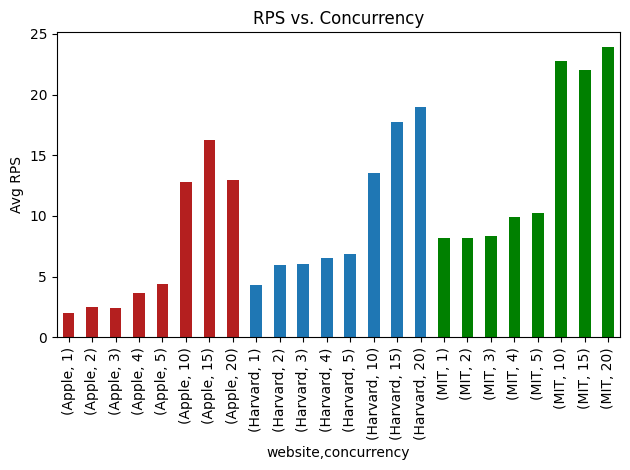
\includegraphics[width=0.48\textwidth]{4_web_conc.png}
        \caption{\small Concurrency VS RPS}
        \label{fig:4_web_conc}
    \end{figure}


\subsubsection{Number of requests VS RPS}
The number of requests sent to a website in a given time interval is another important factor that can affect the website's performance.
As the number of requests increases, the server is forced to handle an higher volume of traffic and the considerations about the 
RPS behavior may not change from the ones discussed above. The results in Figure \ref{fig:4_web_num} show the RPS (averaged across concurrency level)
for each tuple (website, number of requests). As expected there is a positive correlation between the number of requests and the RPS, with the websites
'Apple' and 'MIT' showing a trend quite similar to the one observed in the concurrency analysis. 'Harvard' instead, shows an odd behavior with 
50 requests. According to Figure \ref{fig:4_detailed}, the justification is a dip in the RPS value for 50 requests and 10 concurrency level.
The reasons for this behavior are not clear, therefore a further investigation is necessary.\\

    \begin{figure}[H]
        \centering
        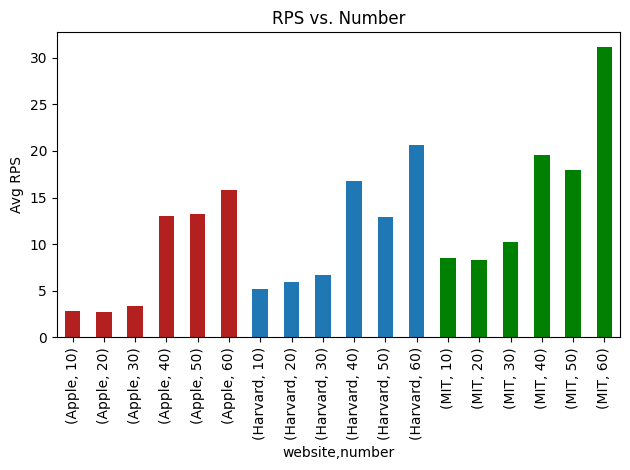
\includegraphics[width=0.48\textwidth]{4_web_num.png}
        \caption{\small Number of requests VS RPS}
        \label{fig:4_web_num}
    \end{figure}

\subsubsection{Overall RPS}
In conclusion to asses a overall performance of the websites, the RPS values for each website were averaged across all the concurrency levels and
number of requests. The results are shown in Figure \ref{fig:4_overall}. The website achieving the highest average RPS is 'MIT', followed by 'Harvard'
and 'Apple'.

    \begin{figure}[H]
        \centering
        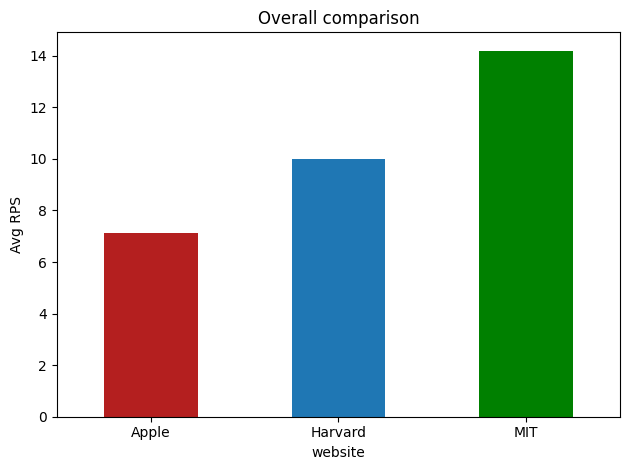
\includegraphics[width=0.48\textwidth]{4_overall.png}
        \caption{\small Overall RPS}
        \label{fig:4_overall}
    \end{figure}


\subsection{Warm-up time impact}
A server hosting a website does not need to operate at its maximum capacity continuously. With proper design and optimization, 
a server can determine when it is necessary to operate at full power and when it can operate in a more energy-efficient manner. 
This approach helps to save energy and reduce operational costs.
However, when transitioning from a lower-power state to full capacity, the server requires a warm-up time to allocate 
resources and reach its optimal performance level. During this warm-up period, the server undergoes initialization processes, 
to prepare itself for handling incoming requests effectively. The warm-up time might impact in a non-negligible way the
performance of the server.\\
\\
\textbf{High Warm-up Time}
A longer warm-up time allows the server to effectively initialize and allocate its resources before the measurement begins. As a 
result, when the measurement period starts, the server is already operating at a high capacity level, enabling it to deliver 
optimal performance.\\
\\
\textbf{Low Warm-up Time}
Conversely to previous situation, a shorter warm-up time can lead the measurement to start before the server reaches
its full potential resulting in lower performance.\\
\\
It is important to note that the impact of warm-up time on server performance can vary due to various factors, such as the specific 
server workload, network conditions, and other environmental variables. As a result, the previously mentioned scenarios regarding the 
relationship between warm-up time and server performance should be interpreted with caution. In this section, we test the warm-up time
impact on different websites performance. For each website different warm-up times were tested with different concurrency levels
(Table \ref{tab:param_warmup}). 

    \begin{table}[H]
        \centering
        \rowcolors{2}{pyblue!25}{white}
            \begin{tabular}{|c|c|}
            \hline
            \rowcolor{pyblue!60}
            \textbf{Parameter} & \textbf{Values} \\
            \hline
            \textbf{Concurrency} & 1, 2, 4, 6, 8, 10 \\
            \textbf{Warm-up (s)} & 2, 4, 6, 8, 10 \\
            \hline
            \end{tabular}
            \caption{\small Parameters warm-up test}
            \label{tab:param_warmup}
    \end{table}

Each experiment was carried out for a duration of 20 seconds, which includes both the actual measurement period and the warm-up time. The used scripts can be consulted 
in the Appendix \ref{sec:scripts}. During 
these experiments, several metrics were recorded to evaluate the performance of the server. The metrics include Requests Per Second (RPS), which measures 
the number of requests processed by the server within a second, Time Per Request (TPR), which calculates the average time taken by the server 
to respond to a single request, and TPR Standard Deviation (SD), which provides an indication of the variability or dispersion of the measured values.
Due to logistic reasons, in this case a 100Mb/s 4G connection from Brescia (BS) was utilized throughout the experiments.\\
In the following sections the results of the experiments are presented and discussed with the help of summarizing charts. To provide an
enhanced perspective of the findings, detailed charts are inserted in the Appendix \ref{sec:detailed_charts}.


\subsubsection{Warm-up time and RPS}
In Figure \ref{fig:5_rps_line}, a consistent pattern is observed across all the websites examined. The Requests Per Second (RPS) metric 
initially increases as the warm-up time is extended, reaching a peak at approximately 6 seconds. However, the delta between the peak and
the neighbors is negligible. Beyond the peak, a slight decrease in RPS can be observed.
The observed behavior can be attributed to several factors. As public websites, the load on these platforms experiences 
significant variations, resulting in fluctuations in the measured results. The complex interaction between user traffic, server capacity,
and network conditions can contribute to the observed patterns in RPS. However, the precise reasons for the slight decrease 
in RPS after the peak are not definitively established and require further investigation.
In conclusion, in the analyzed websites, the RPS metric is not significantly impacted by the warm-up time.\\

    \begin{figure}[H]
        \centering
        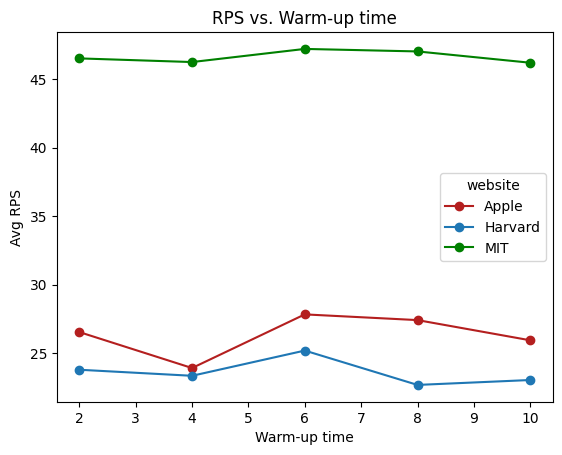
\includegraphics[width=0.48\textwidth]{5_rps_line.png}
        \caption{\small RPS for different warm-up times}
        \label{fig:5_rps_line}
    \end{figure}


\subsubsection{Warm-up time, TPR and SD}
In Figure \ref{fig:5_tpr_line}, the Time Per Request (TPR) metric is shown for different warm-up times. In this case no evident patterns
are observed. It is possible to conclude that in the experiments no correlation appears between the warm-up time and the TPR.\\

    \begin{figure}[H]
        \centering
        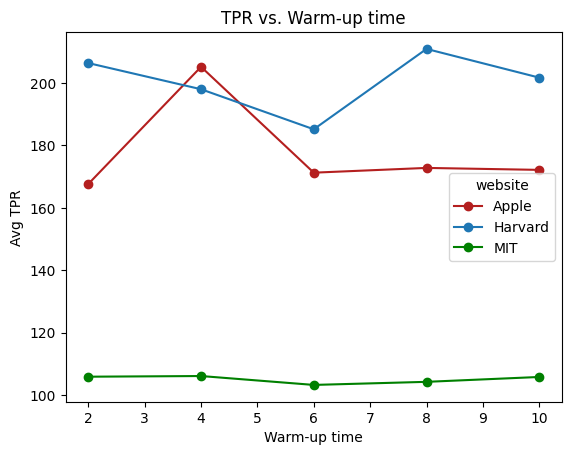
\includegraphics[width=0.48\textwidth]{5_tpr_line.png}
        \caption{\small TPR for different warm-up times}
        \label{fig:5_tpr_line}
    \end{figure}
\noindent
Figure \ref{fig:5_sd_line} presents the TPR Standard Deviation (SD) metric for different warm-up times. Although the pattern may 
not be as pronounced, there appears to be a discernible trend. By dividing the warm-up times into two groups, namely 2 to 5 
seconds and 6 to 10 seconds, it becomes apparent that the SD is higher in the first group. The results indicate that a longer 
warm-up time has a positive impact on the server's performance stability. Indeed, by conceding to the server enough time 
to fully initialize and adapt to the workload, a longer warm-up time facilitates a more stable and predictable performance.

    \begin{figure}[H]
        \centering
        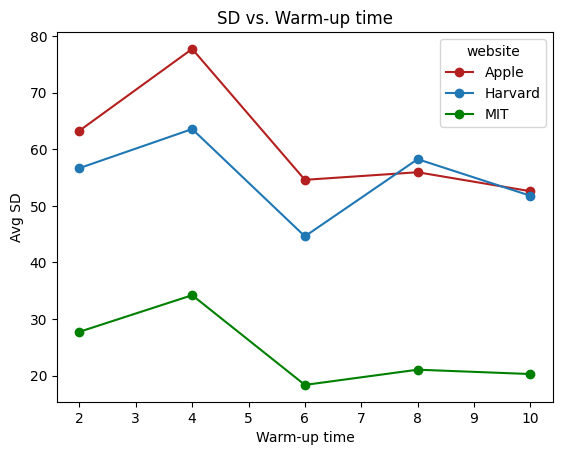
\includegraphics[width=0.48\textwidth]{5_sd_line.png}
        \caption{\small TPR SD for different warm-up times}
        \label{fig:5_sd_line}
    \end{figure}

    In conclusion, while the direct impact of warm-up time on the analyzed websites was not significant within the limitations 
    of the available data, some noteworthy insights into its influence on the RPS and SD metrics were observed. Specifically, 
    a warm-up time of 6 seconds, which accounted for approximately 30\% of the total measurement time, appeared to be associated 
    with a peak in RPS and a decrease in the TPR SD.
    These findings suggest that allocating a sufficient warm-up period for servers can have positive implications for their performance.\\




\subsection{Conclusions}
The findings of this study demonstrate that the number of parallel TCP connections has a significant impact on page load time, 
although there is a diminishing return as the number of connections increases excessively. Based on the results, the default 
choice of six concurrent TCP connections made by browsers appears to be a reasonable selection.

Additionally, caching mechanisms, including the 'Expiration,' 'Validation,' and 'Heuristic' strategies, consistently contribute 
to improved performance. The results clearly indicate the overall benefits of caching, highlighting its importance in reducing 
page load time and enhancing the user experience.

The analysis of different HTTP versions revealed that each new version outperforms its predecessor, regardless of the caching 
mechanism employed. These performance improvements can be attributed to the enhancements introduced in each new version, 
emphasizing the significance of utilizing the latest HTTP protocols.

Regarding the performance analysis of the analyzed websites, it can be concluded that the fastest website is 'MIT,' followed 
by 'Harvard' and 'Apple.'

Although the direct impact of warm-up time on the analyzed websites was found to be not highly relevant, primarily due to 
limited available data, notable observations were made regarding its influence on the RPS (Requests Per Second) and TPR SD (Standard Deviation) 
metrics. Specifically, it was observed that a warm-up time of 6 seconds, comprising approximately 30\% of the total measurement
time, resulted in a peak in RPS and a decrease in TPR SD. These findings suggest that allocating an adequate warm-up period for servers can yield positive implications for their overall performance.

In conclusion, this study provides valuable insights into various aspects of web technologies. The optimal number of parallel TCP 
connections, the importance of caching mechanisms, the superiority of newer HTTP versions, and the potential impact of warm-up 
time allocation for the websites performance assessment.

%°°°°°° Appendix °°°°°°

\end{multicols}
\appendix
\section{Appendix}

\subsection*{Appendix A: Detailed Charts}\label{sec:detailed_charts}

\begin{figure}[H]
    \centering
    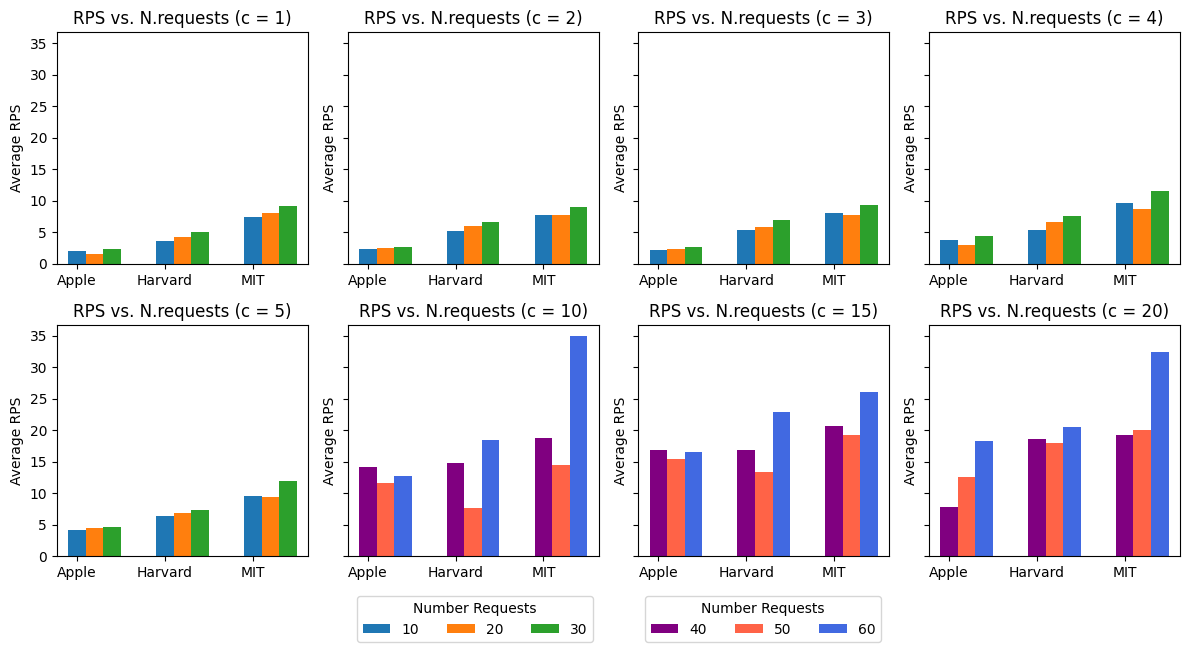
\includegraphics[width=0.90\textwidth]{4_detailed.png}
    \caption{\small Detailed analysis RPS vs Number of requests and Concurrency level}
    \label{fig:4_detailed}
\end{figure}

\begin{figure}[H]
    \centering
    \includegraphics[width=0.90\textwidth]{5_RPS_detailed.png}
    \caption{\small RPS and Warm-up time for different concurrency levels}
    \label{fig:5_RPS_detailed}
\end{figure}

\begin{figure}[H]
    \centering
    \includegraphics[width=0.90\textwidth]{5_TPR_detailed.png}
    \caption{\small TPR and Warm-up time for different concurrency levels}
    \label{fig:5_TPR_detailed}
\end{figure}

\begin{figure}[H]
    \centering
    \includegraphics[width=0.90\textwidth]{5_SD_detailed.png}
    \caption{\small SD and Warm-up time for different concurrency levels}
    \label{fig:5_SD_detailed}
\end{figure}


\subsection*{Appendix B: Scripts}\label{sec:scripts}

\begin{figure}[H]
    \centering
    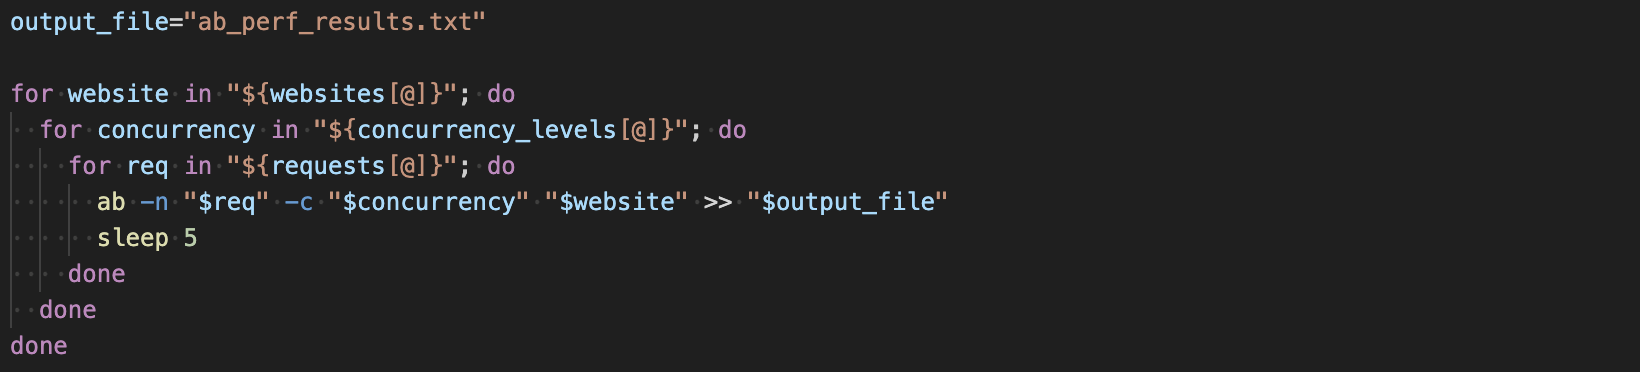
\includegraphics[width=0.90\textwidth]{4_ab_perf_script.png}
    \caption{\small Bash script for ab experiments}
    \label{fig:4_ab_perf_script}
\end{figure}

\begin{figure}[H]
    \centering
    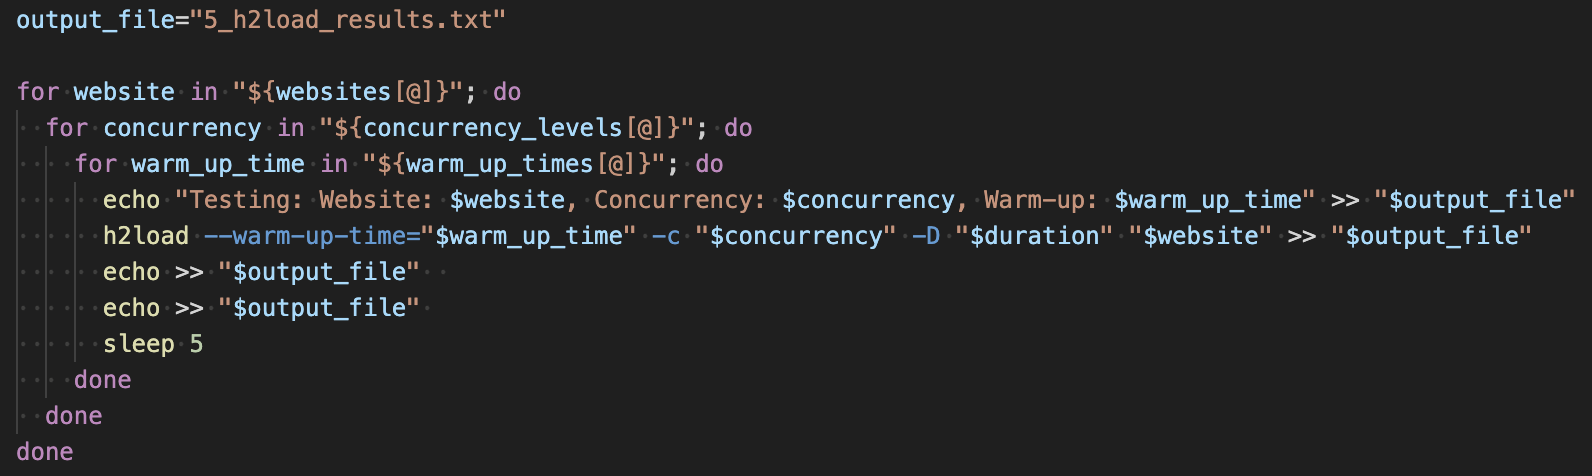
\includegraphics[width=0.90\textwidth]{5_h2load_script.png}
    \caption{\small Bash script for h2load experiments}
    \label{fig:5_h2load_script}
\end{figure}


\begin{multicols}{2}



%°°°°°° Mail °°°°°°




%°°°°°°°°°°°°°°°°°°°°°°°°°°°°°°°°°END BODY OF THE DOCUMENT°°°°°°°°°°°°°°°°°°°°°°°°°°°°°°°°


\end{multicols}

%\bibliographystyle{unsrtnat}
%\bibliography{References}
\end{document}